Fitting the anomalous couplings one at a time while fixing the other couplings
to the Standard Model values, we get the following results:

%% Minuit2Minimizer: Minimize with max iterations 3500 edmval 1 strategy 1
%% Minuit2Minimizer : Valid minimum - status = 0
%% FVAL  = -1597.8426506188207
%% Edm   = 7.67985758123812141e-06
%% Nfcn  = 98
%% n_dy	  = 15.8771	 +/-  12.2352	(limited)
%% n_top	  = 123.885	 +/-  39.0584	(limited)
%% n_wjets	  = 125.305	 +/-  37.5327	(limited)
%% n_ww	  = 818.001	 +/-  70.3764	(limited)
%% n_wz	  = 19.0333	 +/-  3.71018	(limited)
%% n_zz	  = 10.6555	 +/-  1.95391	(limited)
%% x_par	  = 0.00173999	 +/-  0.0372007	(limited)
%% Info in <Minuit2>: MnMinos Parameter is at Lower limit. : par = 0
%% Minos:  Parameter  is at Lower limit.
%% Minos: Lower error for parameter 0  :  -12.9521
%% Minos: Upper error for parameter 0  :  13.17
%% Minos: Lower error for parameter 1  :  -39.0776
%% Minos: Upper error for parameter 1  :  39.5969
%% Minos: Lower error for parameter 2  :  -37.8738
%% Minos: Upper error for parameter 2  :  38.115
%% Minos: Lower error for parameter 3  :  -70.1309
%% Minos: Upper error for parameter 3  :  70.713
%% Minos: Lower error for parameter 4  :  -3.72022
%% Minos: Upper error for parameter 4  :  3.72172
%% Minos: Lower error for parameter 5  :  -1.95866
%% Minos: Upper error for parameter 5  :  1.959
%% Minos: Lower error for parameter 6  :  -0.0351527
%% Minos: Upper error for parameter 6  :  0.0336279

%% Minuit2Minimizer: Minimize with max iterations 3500 edmval 1 strategy 1
%% Minuit2Minimizer : Valid minimum - status = 0
%% FVAL  = -1597.8541092969524
%% Edm   = 1.9043130473987436e-05
%% Nfcn  = 88
%% n_dy	  = 15.893	 +/-  12.2342	(limited)
%% n_top	  = 123.969	 +/-  39.047	(limited)
%% n_wjets	  = 125.389	 +/-  37.5327	(limited)
%% n_ww	  = 818.107	 +/-  70.4418	(limited)
%% n_wz	  = 19.0347	 +/-  3.71014	(limited)
%% n_zz	  = 10.6559	 +/-  1.9539	(limited)
%% y_par	  = 0.0053376	 +/-  0.0591742	(limited)
%% Info in <Minuit2>: MnMinos Parameter is at Lower limit. : par = 0
%% Minos:  Parameter  is at Lower limit.
%% Minos: Lower error for parameter 0  :  -12.968
%% Minos: Upper error for parameter 0  :  13.1525
%% Minos: Lower error for parameter 1  :  -39.0665
%% Minos: Upper error for parameter 1  :  39.5797
%% Minos: Lower error for parameter 2  :  -37.9446
%% Minos: Upper error for parameter 2  :  38.0455
%% Minos: Lower error for parameter 3  :  -69.9994
%% Minos: Upper error for parameter 3  :  70.983
%% Minos: Lower error for parameter 4  :  -3.72148
%% Minos: Upper error for parameter 4  :  3.72048
%% Minos: Lower error for parameter 5  :  -1.9589
%% Minos: Upper error for parameter 5  :  1.95877
%% Minos: Lower error for parameter 6  :  -0.0565435
%% Minos: Upper error for parameter 6  :  0.0545804

%% Minuit2Minimizer: Minimize with max iterations 3500 edmval 1 strategy 1
%% Minuit2Minimizer : Valid minimum - status = 0
%% FVAL  = -1603.51147260254811
%% Edm   = 1.20113893713908417e-05
%% Nfcn  = 92
%% n_dy	  = 14.6808	 +/-  12.1947	(limited)
%% n_top	  = 130.388	 +/-  38.6532	(limited)
%% n_wjets	  = 116.58	 +/-  37.9489	(limited)
%% n_ww	  = 822.541	 +/-  70.2736	(limited)
%% n_wz	  = 18.9885	 +/-  3.71024	(limited)
%% n_zz	  = 10.6654	 +/-  1.95387	(limited)
%% y_par	  = -0.00452245	 +/-  0.147562	(limited)
%% Info in <Minuit2>: MnMinos Parameter is at Lower limit. : par = 0
%% Minos:  Parameter  is at Lower limit.
%% Minos: Lower error for parameter 0  :  -11.7558
%% Minos: Upper error for parameter 0  :  13.1895
%% Minos: Lower error for parameter 1  :  -38.749
%% Minos: Upper error for parameter 1  :  39.0973
%% Minos: Lower error for parameter 2  :  -38.3649
%% Minos: Upper error for parameter 2  :  38.5348
%% Minos: Lower error for parameter 3  :  -70.0857
%% Minos: Upper error for parameter 3  :  70.5636
%% Minos: Lower error for parameter 4  :  -3.72106
%% Minos: Upper error for parameter 4  :  3.72117
%% Minos: Lower error for parameter 5  :  -1.95884
%% Minos: Upper error for parameter 5  :  1.95877
%% Minos: Lower error for parameter 6  :  -0.144142
%% Minos: Upper error for parameter 6  :  0.128754


%% \begin{align}
%%   \lambda_{Z} &= 0.00\pm0.19, ~95\%~\mathrm{C.L.} \\ 
%%   \Delta g^Z_1 &= 0.01\pm0.30, ~95\%~\mathrm{C.L.}\\
%%   \Delta\kappa_\gamma &= 0.02\pm0.63, ~95\%~\mathrm{C.L.}\\
%% \end{align}

%% \fixme{What do we do with coverage? Ignore for now}

%% Sampling \wwll\ Monte Carlo events we find that within the reported 95\%
%% confidence limits $\lambda_{Z}$ contained $97\pm1$\% and
%% $\Delta\kappa_{Z}$ contained $94\pm1$\% of the test samples.

Systematic uncertainties were included in the fit as Gaussian
constraints.

Final exclusion limits for anomalous couplings are:
\begin{align}
  \lambda_{Z}: [-0.04,0.04]~95\%~\mathrm{C.L.}\\ 
  \Delta g^{Z}_1: [-0.07,0.08]~95\%~\mathrm{C.L.}\\
  \Delta\kappa_\gamma: [-0.21,0.17]~95\%~\mathrm{C.L.}\\
\end{align}
The results include the scale correction of 20-30\% observed in the validation studies.

Figure~\ref{fig:contour} shows 2D confidence limit contour plots for
anomalous couplings.

\begin{figure}[tp]
  \centerline{
    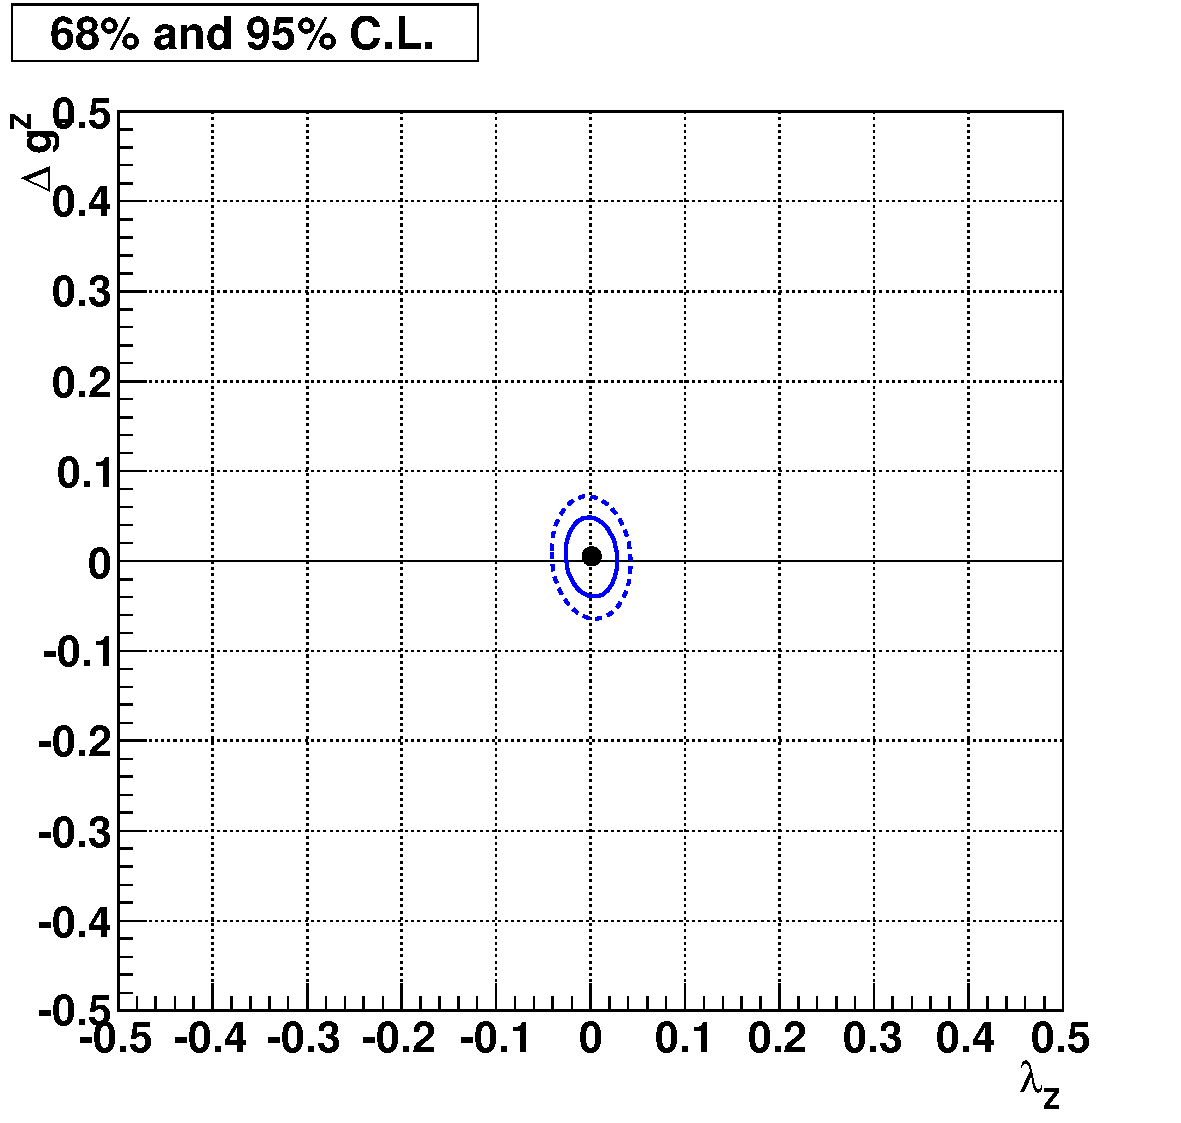
\includegraphics[width=0.5\textwidth]{figures/lz_dgz_contourplot}
    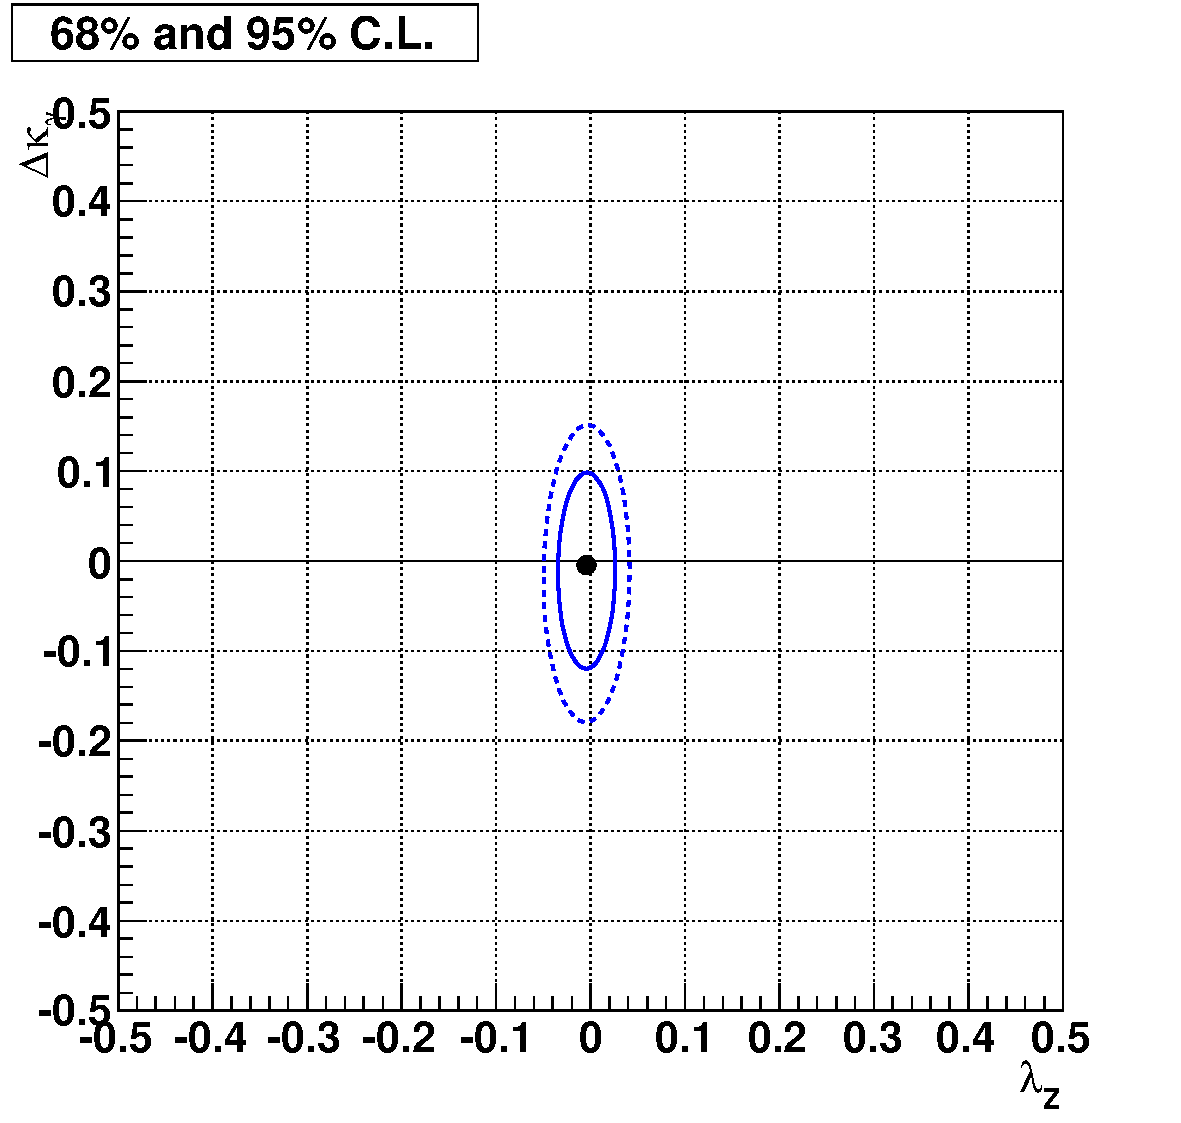
\includegraphics[width=0.5\textwidth]{figures/lz_dkg_contourplot}
  }

  \caption[Contour plots for data] {aTGC 68\% and 95\% C.L. contour
    plots for a model without form factors for \intlumi of data.}
  \label{fig:contour}
\end{figure}

